\section{Compatibility of the three trace Paley--Wiener theorems}\label{sec:pwcomparison}
The purpose of this section is to compare restriction of the spectrum with enlargement of the test-function space. We work with $G=\mathrm{SL}_2(F)$, where the residual characteristic is odd, and normalized induction $I(\chi)$ from the upper triangular Borel. All trace spaces below are vector spaces, not algebras under pointwise multiplication.

\subsection{The comparison maps}
Write $H=C_c^\infty(G)$ and $S=\mathcal C(G)$ for the Hecke and Harish-Chandra Schwartz algebras. For $X=\mathrm{ad},u,t$, let $R_X$ be the complex vector space freely generated by the corresponding irreducible admissible, unitarizable, or tempered representations. Trace additivity identifies $R_{\mathrm{ad}}$ with the complexified finite-length Grothendieck group. Put $T_X(f)(\pi)=\operatorname{tr}\pi(f)$, and write $E_X=T_X(H)$ and $E_S=T_t(S)$. In particular $E_t$ means compact-support tempered trace data, not the Schwartz image.

\begin{center}
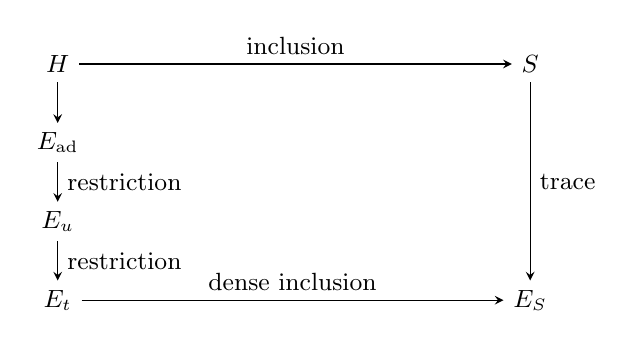
\begin{tikzpicture}[>=stealth, every node/.style={font=\small}]
\node (h) at (0,3) {$H$}; \node (s) at (6,3) {$S$};
\node (a) at (0,2) {$E_{\mathrm{ad}}$};
\node (u) at (0,1) {$E_u$};
\node (t) at (0,0) {$E_t$}; \node (e) at (6,0) {$E_S$};
\draw[->] (h)--node[above]{inclusion}(s);
\draw[->] (h)--(a); \draw[->] (a)--node[right]{restriction}(u);
\draw[->] (u)--node[right]{restriction}(t);
\draw[->] (s)--node[right]{trace}(e);
\draw[->] (t)--node[above]{dense inclusion}(e);
\end{tikzpicture}
\end{center}

\begin{theorem}\label{thm:pwcomparison}
The restriction maps $E_{\mathrm{ad}}\to E_u\to E_t$ are vector-space isomorphisms.
\end{theorem}
\begin{proof}
Surjectivity follows from the definitions. Suppose that $f\in H$ has zero trace on every irreducible tempered representation. Fix a smooth character $\xi$ of $\mathcal O_F^\times$ and put $\chi_{\xi,z}(\varpi^m a)=z^m\xi(a)$, where $z\in\mathbb C^\times$. The function
\[
P_{\xi,f}(z)=\operatorname{tr} I(\chi_{\xi,z})(f)
\]
is a Laurent polynomial by regularity of induced traces (the compact realization also gives this directly). For $|z|=1$ every constituent of the normalized induction is tempered. Additivity of traces gives $P_{\xi,f}(z)=0$ on the circle. Multiplying by a sufficiently large power of $z$ gives an ordinary polynomial with infinitely many roots, so $P_{\xi,f}$ vanishes identically.

The rank-one classification now gives vanishing on every irreducible principal series. The constituents at nontrivial quadratic inducing characters are already tempered. At the remaining reducibility point use $[I(|\cdot|)]=[\mathbf 1]+[\mathrm{St}]$. Since the Steinberg trace is zero, the trivial trace is zero as well. Supercuspidals are tempered because the center is finite. Thus every admissible irreducible trace vanishes, proving injectivity of both restrictions.
\end{proof}

By Kazhdan's density theorem \cite{Ka86}, the common kernel is the linear commutator span $[H,H]$. Consequently all three compact-support trace images identify with the algebraic cocenter $H/[H,H]$. This does not imply injectivity of the trace map on $H$ itself.

\subsection{Explicit coordinates and the unitary theorem}
Write $W$ for inversion on $\mathbb C^\times$, and $u=z+z^{-1}$. The good-functional trace Paley--Wiener theorem \cite{BDK86} requires uniform compact-open level and regularity on induced families. In rank one the only proper Levi is the diagonal torus. For a fixed principal-series block, regularity is exactly the Laurent-polynomial requirement on the total induced trace. The level condition is automatic for the proposed data in finitely many blocks: choose a principal congruence subgroup fixing the inducing compact model at that level and nonzero vectors in each exceptional constituent, and decrease it to accommodate the finitely many supercuspidals. For generic induced representations the fixed-vector dimension is independent of unramified twist. Thus the following coordinate descriptions follow from the classical classification and the good-functional theorem.

\begin{center}
\begin{tabular}{lll}
\hline
Block & $E_{\mathrm{ad}}\simeq E_u\simeq E_t$ & $E_S$ (see below)\\
\hline
Supercuspidal & $\mathbb C$ & $\mathbb C$\\
$\xi^2\ne1$ & $\mathbb C[z,z^{-1}]$ & $C^\infty(S^1)$\\
$\xi^2=1,\ \xi\ne1$ & $\mathbb C[u]\oplus\mathbb C^2$ & $C^\infty(S^1)^W\oplus\mathbb C^2$\\
$\xi=1$ & $\mathbb C[u]\oplus\mathbb C^2$ & $C^\infty(S^1)^W\oplus\mathbb C^2$\\
\hline
\end{tabular}
\end{center}
For $\xi^2\ne1$ choose one of the two inverse restrictions to units. For ramified quadratic $\xi$ the exceptional coordinates are the differences of the two constituent traces at each of $z=1,-1$. For $\xi=1$, use $d=\phi(\pi_+)-\phi(\pi_-)$ at $z=-1$ and $b=\phi(\mathrm{St})$. Set $c=q+q^{-1}$. The remaining traces are
\[
\phi(\pi_\pm)=\tfrac12(Q(-2)\pm d),\qquad
\phi(\mathbf 1)=Q(c)-b.
\]
Here $Q(u)$ is the total induced trace. In particular the same polynomial governs both the unitary principal series ($-2\le u\le2$) and complementary series ($2<u<c$). These conditions are necessary and sufficient within this block: extend the polynomial to the complex torus, impose the displayed sums at reducibility, and apply the good-functional theorem. This is an explicit unitary trace Paley--Wiener theorem, not an independent assumption.

\begin{example}
For $F=\mathbb Q_3$, take $Q(u)=u^2-2$, the Laurent polynomial $z^2+z^{-2}$. The total quadratic trace is $2$, and the trivial plus Steinberg trace is $82/9$. The individual traces depend on $d,b$. More generally $z^n+z^{-n}=2T_n(u/2)$, where $T_n$ is the Chebyshev polynomial.
\end{example}
\begin{center}
\begin{tikzpicture}[x=1.35cm,y=.38cm,>=stealth]
\draw[->] (-2.3,0)--(3.65,0) node[right]{$u$};
\draw[->] (0,-2.6)--(0,10) node[above]{$Q$};
\draw[teal,thick,domain=-2:2,samples=60] plot (\x,{\x*\x-2});
\draw[orange!80!black,thick,domain=2:3.333,samples=60] plot (\x,{\x*\x-2});
\foreach \x/\l in {-2/-2,2/2,3.333/{10/3}} {\draw (\x,.15)--(\x,-.15) node[below]{$\l$};}
\node[teal] at (-1.5,5) {tempered};
\node[orange!80!black] at (2.6,7) {complementary};
\end{tikzpicture}
\end{center}

\subsection{The Schwartz comparison and completion}
Arthur's trace Paley--Wiener theorem for Schwartz functions \cite[p.~174]{Ar94} gives a continuous open surjection onto smooth data on virtual tempered character parameter spaces. The rank-one coordinate model in the last column above uses the induced unitary circle, the independent difference of quadratic constituents at each reducibility point, and the independent Steinberg trace. In particular the unramified comparison is $(Q,d,b)\mapsto(Q|_{[-2,2]},d,b)$. The Steinberg representation is discrete series and contributes its own coordinate, not a value on the circle. The precise identification with Arthur's topology, including the normalization of virtual characters and global level filtration, is a remaining source-verification task (Remark 2026.1). The following density conclusion does not require that explicit identification.

\begin{theorem}\label{thm:pwcompletion}
The compact-support trace image $E_t$ is dense in $E_S$ with Arthur's quotient topology.
\end{theorem}
\begin{proof}
Compactly supported smooth functions are dense in $S$: on a fixed compact-open bi-invariant Schwartz stage, truncate on compact unions of double cosets with length bounded by $m$. The error in each weighted supremum seminorm tends to zero, by using a seminorm with one additional power of the length. Continuity and surjectivity of Arthur's trace map now give density.
\end{proof}
If the blockwise Fréchet models and their locally convex direct sum are identified with the Schwartz image, its completeness follows from completeness of those spaces. In that topology the completion of $E_t$ is $E_S$. This last global identification is recorded separately rather than assumed. On each proposed block, Fourier partial sums prove density in every smooth seminorm. Weyl averaging preserves convergence and exceptional coordinates may be held fixed.

\begin{center}
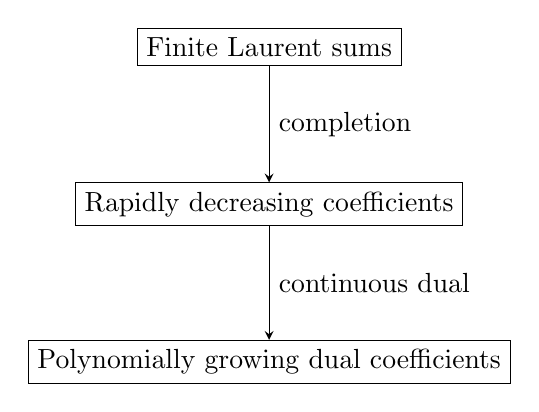
\begin{tikzpicture}[>=stealth]
\node[draw] (p) at (0,2) {Finite Laurent sums};
\node[draw] (s) at (0,0) {Rapidly decreasing coefficients};
\node[draw] (d) at (0,-2) {Polynomially growing dual coefficients};
\draw[->] (p)--node[right]{completion}(s);
\draw[->] (s)--node[right]{continuous dual}(d);
\end{tikzpicture}
\end{center}

\subsection{Instability of algebraic continuation}
Uniqueness of continuation must not be confused with continuity. The following elementary spectral calculation applies to the proposed smooth block model.
\begin{theorem}\label{thm:pwinstability}
For $s_0>0$, put $P_n(z)=q^{-ns_0}(z^n+z^{-n})$. Then $P_n|_{S^1}\to0$ in $C^\infty(S^1)$, but $P_n(q^{-s_0})\to1$.
\end{theorem}
\begin{proof}
The $k$th angular derivative has supremum at most $2n^kq^{-ns_0}$, which tends to zero for each $k$. At $q^{-s_0}$ the value is $1+q^{-2ns_0}$.
\end{proof}
Take $0<s_0<1$ for a complementary-series trace, or $s_0=1$ with $b=0$ for the trivial trace. Set the other exceptional coordinate to zero. By the admissible trace theorem these data have Hecke-algebra preimages. Consequently non-tempered evaluation is discontinuous for the smooth spectral topology. Its interpretation in Arthur's topology uses the identification in Remark 2026.1. This separates algebraic determination by tempered traces from continuous determination after completion.

\begin{center}
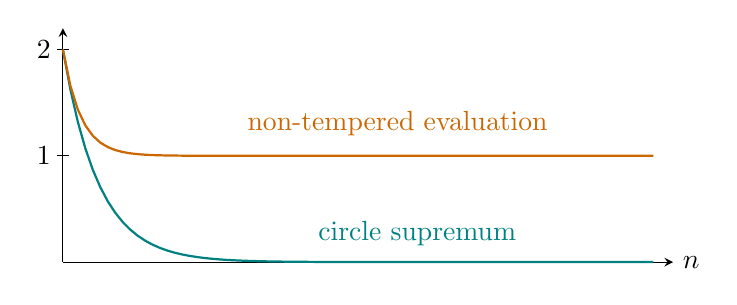
\begin{tikzpicture}[x=.25cm,y=1.35cm,>=stealth]
\draw[->] (0,0)--(31,0) node[right]{$n$};
\draw[->] (0,0)--(0,2.2);
\foreach \y in {1,2} {\draw (-.3,\y)--(.3,\y) node[left,xshift=-3pt]{$\y$};}
\draw[teal,thick,domain=0:30,samples=80] plot (\x,{2*3^(-\x/2)});
\draw[orange!80!black,thick,domain=0:30,samples=80] plot (\x,{1+3^(-\x)});
\node[teal] at (18,.27) {circle supremum};
\node[orange!80!black] at (17,1.3) {non-tempered evaluation};
\end{tikzpicture}
\end{center}

\subsection{Intermediate analytic spaces}
For $r>1$ put $A_r=\{z:r^{-1}<|z|<r\}$. The compact-open topology on $\mathcal O(A_r)^W$ makes evaluation at $q^{-s}$ continuous for $q^s<r$. Laurent polynomials are dense by Laurent expansion on compact subannuli. Cauchy's estimates give exponential decay of the Laurent coefficients at every rate strictly below $r$. For holomorphic functions on $\mathbb C^\times$ this holds at every finite rate. For smooth circle functions it is replaced by rapid polynomial decay. The exceptional coordinates can be appended as independent finite-dimensional summands; a non-tempered constituent trace only extends if the corresponding evaluation is continuous.

\begin{center}
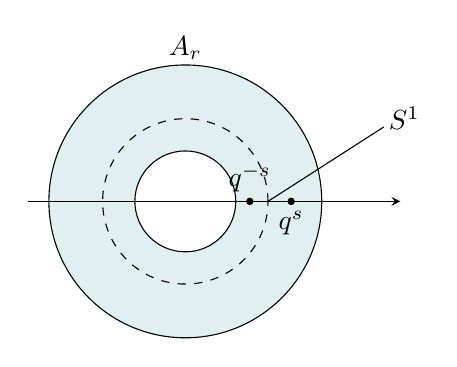
\begin{tikzpicture}[>=stealth,scale=1.05]
\fill[teal!12,even odd rule] (0,0) circle (1.65) (0,0) circle (.61);
\draw (0,0) circle (1.65); \draw (0,0) circle (.61);
\draw[dashed] (0,0) circle (1);
\draw[->] (-1.9,0)--(2.6,0);
\fill (.78,0) circle (.045) node[above]{$q^{-s}$};
\fill (1.28,0) circle (.045) node[below]{$q^s$};
\node at (0,1.85) {$A_r$};
\node at (2.65,1) {$S^1$};
\draw (1,0)--(2.4,.9);
\end{tikzpicture}
\end{center}
A research question is whether the trace images of Harish-Chandra $L^p$-Schwartz spaces, $0<p<2$, with decay controlled by $\Xi^{2/p}$ and all polynomial length weights, admit descriptions on such annuli with boundary regularity. Neither a radius formula nor surjectivity is asserted here.

\subsection{Duality and invariant distributions}
On the unramified polynomial summand use $B_0=1$, $B_n=z^n+z^{-n}$ for $n\ge1$. The locally convex inductive limit of bounded-degree polynomial spaces has every linear functional continuous. The inherited smooth topology is strictly weaker.
\begin{theorem}\label{thm:pwdual}
A functional $\ell$ on $\mathbb C[u]\oplus\mathbb C^2$ extends continuously to $C^\infty(S^1)^W\oplus\mathbb C^2$ if and only if $|\ell(B_n,0,0)|\le C(1+n)^N$ for all $n\ge0$ and some $C,N$.
\end{theorem}
\begin{proof}
Continuity bounds $\ell$ by finitely many smooth seminorms, and the $k$th derivatives of $B_n$ have supremum at most $2n^k$ for $n\ge1$. Conversely the coefficients in $h=a_0+\sum_{n\ge1}a_nB_n$ decrease rapidly, so the sum $\sum a_n\ell(B_n,0,0)$ converges absolutely and is bounded by a smooth seminorm by integration by parts. Append the two finite-dimensional functionals. Density proves uniqueness.
\end{proof}
The constant mode is independent and must be retained. Evaluation at $1$ has coefficients $2$ for $n\ge1$, evaluation at $-1$ has $2(-1)^n$, and the second angular derivative at $1$ has $-2n^2$. Complementary-series evaluation grows as $q^{ns}+q^{-ns}$ and fails the criterion. The trivial character similarly fails, whereas the independent Steinberg coordinate satisfies it.

Globally the anticipated topology is the locally convex direct sum of the block spaces, not their product. Its continuous dual is the product of the block duals. Bernstein finiteness at fixed compact-open level and the converse control of block stages must be checked in the Schwartz setting. No uniform growth estimate across all blocks is required if the direct-sum topology holds.

\subsection{Cocenters and the remaining research program}
The algebraic cocenter is $HH_0(H)$. The natural topological counterpart is $S/\overline{[S,S]}$. Identifying this with the Schwartz trace image requires the equality of its trace kernel with the closed commutator span; the trace theorem alone does not assert that equality. This modern interpretation motivates the comparison with Solleveld's work on Hochschild homology of reductive $p$-adic group algebras.
\begin{center}
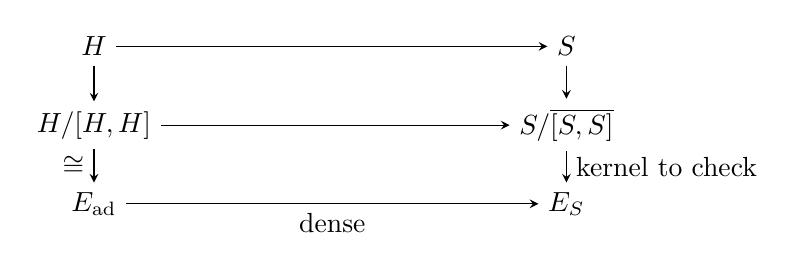
\begin{tikzpicture}[>=stealth]
\node (h) at (0,2) {$H$}; \node (s) at (6,2) {$S$};
\node (c) at (0,1) {$H/[H,H]$};
\node (d) at (6,1) {$S/\overline{[S,S]}$};
\node (a) at (0,0) {$E_{\mathrm{ad}}$}; \node (b) at (6,0) {$E_S$};
\draw[->] (h)--(s); \draw[->] (h)--(c); \draw[->] (s)--(d);
\draw[->] (c)--(d); \draw[->] (c)--node[left]{$\cong$}(a);
\draw[->] (d)--node[right]{kernel to check}(b);
\draw[->] (a)--node[below]{dense}(b);
\end{tikzpicture}
\end{center}
The priorities are to verify Arthur's virtual-character normalization and topology in rank one, identify the global completion and closed commutator kernel, and investigate intermediate holomorphic trace spaces. The algebraic comparison and elementary spectral estimates above are proved subject to their stated classical inputs; novelty relative to the literature is not claimed.
